
% Perspectives for HET physics studies at a muon-hadron collider at CERN
% HELP4CERN Study Group
% DIS 2026, 4-8 May 2026, Bologna, Italy

\documentclass[a4paper,11pt]{article}

\usepackage{pos}
\usepackage{amsmath}
\usepackage{booktabs}
\usepackage{placeins}
\usepackage{tikz-feynman}
\tikzfeynmanset{compat=1.1.0,warn luatex=false,
 medium/.style={/tikz/node distance=1.5cm}}


\newcommand{\lhmuc}{LH$\mu$C}


\title{Perspectives for HET physics studies at a muon-hadron collider at CERN}
\ShortTitle{HET physics at a muon-hadron collider at CERN}
\author*[]{Hamzeh Khanpour}
\onbehalf*{(on behalf of HELP4CERN Study Group)}
\affiliation[]{AGH University of Krakow, Faculty of Physics and Applied Computer Science,
Al. Mickiewicza 30, 30-055 Krak\'ow, Poland.}
\emailAdd{hamzeh.khanpour@cern.ch}


\abstract{%
A muon-hadron collider at CERN would extend lepton-proton collisions 
into the multi-TeV regime and provide a complementary programme of Higgs, 
electroweak and top (HET) physics. We present the HELP4CERN prospects for 0.5, 1 and 2~TeV muon 
beams colliding with 7~TeV protons, corresponding to centre-of-mass energies of approximately 3.7, 5.3 and 7.5~TeV. 
The production benchmarks show substantial gains over the LHeC, particularly for 
top-quark final states.  
The accessible deep-inelastic-scattering (DIS) phase space and inclusive production 
rates provide the basis for the physics programme. Particular attention is given to a 
dedicated charged-current $h\to b\bar b$ study and an exploratory combined Higgs-coupling fit, 
distinguishing statistical rate precision from coupling constraints that depend on external information 
and fit assumptions. Electroweak and top measurements, photon-induced production, and muon-coupled new-physics 
channels offer complementary directions.  }


\FullConference{33rd International Workshop on Deep Inelastic Scattering and Related Subjects (DIS2026)\\
4-8 May 2026, Bologna, Italy}



\begin{document}
\maketitle


%===============================
\section{Collider benchmarks and HET production rates}\label{sec:setup}
%===============================


The proposed \lhmuc\ would collide positive muons with the 7~TeV proton beam of 
the High-Luminosity LHC, extending the lepton-hadron programme beyond the 
electron-beam configurations of the LHeC~\cite{Akturk:2025ubm,LHeC:2020van,Ahmadova:2025vzd}. 
Its higher collision energy opens additional phase space for Higgs, 
electroweak and top (HET) production, with complementary photon-induced and muon-coupled 
new-physics channels.      
Table~\ref{tab:rates} gives the inclusive production cross-sections for the Higgs and top-quark at the \lhmuc.\ 
The energy dependence is particularly pronounced for heavy final states:  
relative to the 50~GeV LHeC entries, the 500~GeV and 1~TeV muon configurations 
increase the single-top cross-section by factors of approximately 7-13 and the 
top-pair cross-section by 32-69. These comparisons describe the stated production 
benchmarks; experimental precision additionally depends on luminosity, selection and uncertainties. 


%-----------------------------------------
\begin{table}[htbp]
\centering
\small
\setlength{\tabcolsep}{6pt}
\renewcommand{\arraystretch}{1.18}
\begin{tabular}{lcccc}
\toprule
Process & 20~GeV & 50~GeV & 500~GeV & 1~TeV\\
& LHeC & LHeC & \lhmuc & \lhmuc\\
\midrule
$\sigma(\ell p\to\nu_\ell H+\mathrm{jet}+X)$ [fb]
& 52 & 164 & 438 & 731\\
$\sigma(\ell p\to\ell H+\mathrm{jet}+X)$ [fb]
& 5.6 & 19 & 135 & 221\\
$\sigma(\ell p\to\ell t\bar t+X)$ [pb]
& 0.0015 & 0.0323 & 1.03 & 2.23\\
$\sigma(\ell p\to\nu_\ell t+X)$ [pb]
& 0.55 & 2.89 & 21.26 & 36.77\\
\bottomrule
\end{tabular}
\caption{Benchmark inclusive production cross-sections for
Higgs-boson, top-quark-pair, and single-top production at the
LHeC and \lhmuc. 
In the LHeC cases an 80\% electron beam polarisation is assumed~\cite{Andre:2025iar}.}
\label{tab:rates}
\end{table}
%-----------------------------------------

The three working points in Table~\ref{tab:benchmarks} span collision energies 
from 3.7 to 7.5~TeV. Already the first option enters the multi-TeV regime; 
the nominal baseline combines increased energy with a larger benchmark sample, 
while the second option further extends the accessible momentum transfer and final-state masses. 


%-----------------------------------------
\begin{table}[htbp]
\centering
\small
\setlength{\tabcolsep}{6pt}
\renewcommand{\arraystretch}{1.18}
\begin{tabular}{lcccc}
\toprule
Configuration & $E_\mu$ & $E_p$ & $\sqrt{s_{\mu p}}$ & $\mathcal{L}_{\mathrm{int}}$\\
\midrule
First option & 500~GeV & 7~TeV & 3.7~TeV & $250~\mathrm{fb}^{-1}$\\
Nominal baseline & 1~TeV & 7~TeV & 5.3~TeV & $1000~\mathrm{fb}^{-1}$\\
Second option & 2~TeV & 7~TeV & 7.5~TeV & $1000~\mathrm{fb}^{-1}$\\
\bottomrule
\end{tabular}
\caption{Benchmark \lhmuc\ working points based on the HELP4CERN
studies~\cite{HELP4CERN}.}
\label{tab:benchmarks}
\end{table}
%-----------------------------------------

These working points illustrate the potential of the \lhmuc\ physics
programme. Already with a 500~GeV muon beam, collisions with 7~TeV
protons enter the multi-TeV centre-of-mass regime, providing a basis
for competitive studies of Higgs production, electroweak interactions,
top-quark processes, photon-induced reactions, and representative
scenarios beyond the Standard Model. The nominal baseline combines
a higher collision energy with a larger benchmark data sample,
supporting more demanding precision measurements and searches.
The 2~TeV muon-beam option further extends the accessible momentum
transfer and final-state invariant masses. Together, these
configurations provide a framework for examining how the physics
opportunities develop with collision energy and integrated luminosity. 

Figure~\ref{fig:coverage} illustrates the enlarged $(x_{\mathrm{Bj}},Q^2)$ coverage. 
The high-$Q^2$ reach motivates electroweak tests in deep-inelastic scattering (DIS), 
alongside the hard-scattering phase space available for HET production. 
The broader QCD programme also supplies proton-structure information relevant 
to precision measurements at hadron colliders~\cite{Ahmadova:2025vzd}. 


%-----------------------------------------
\begin{figure}[tbp]
\centering
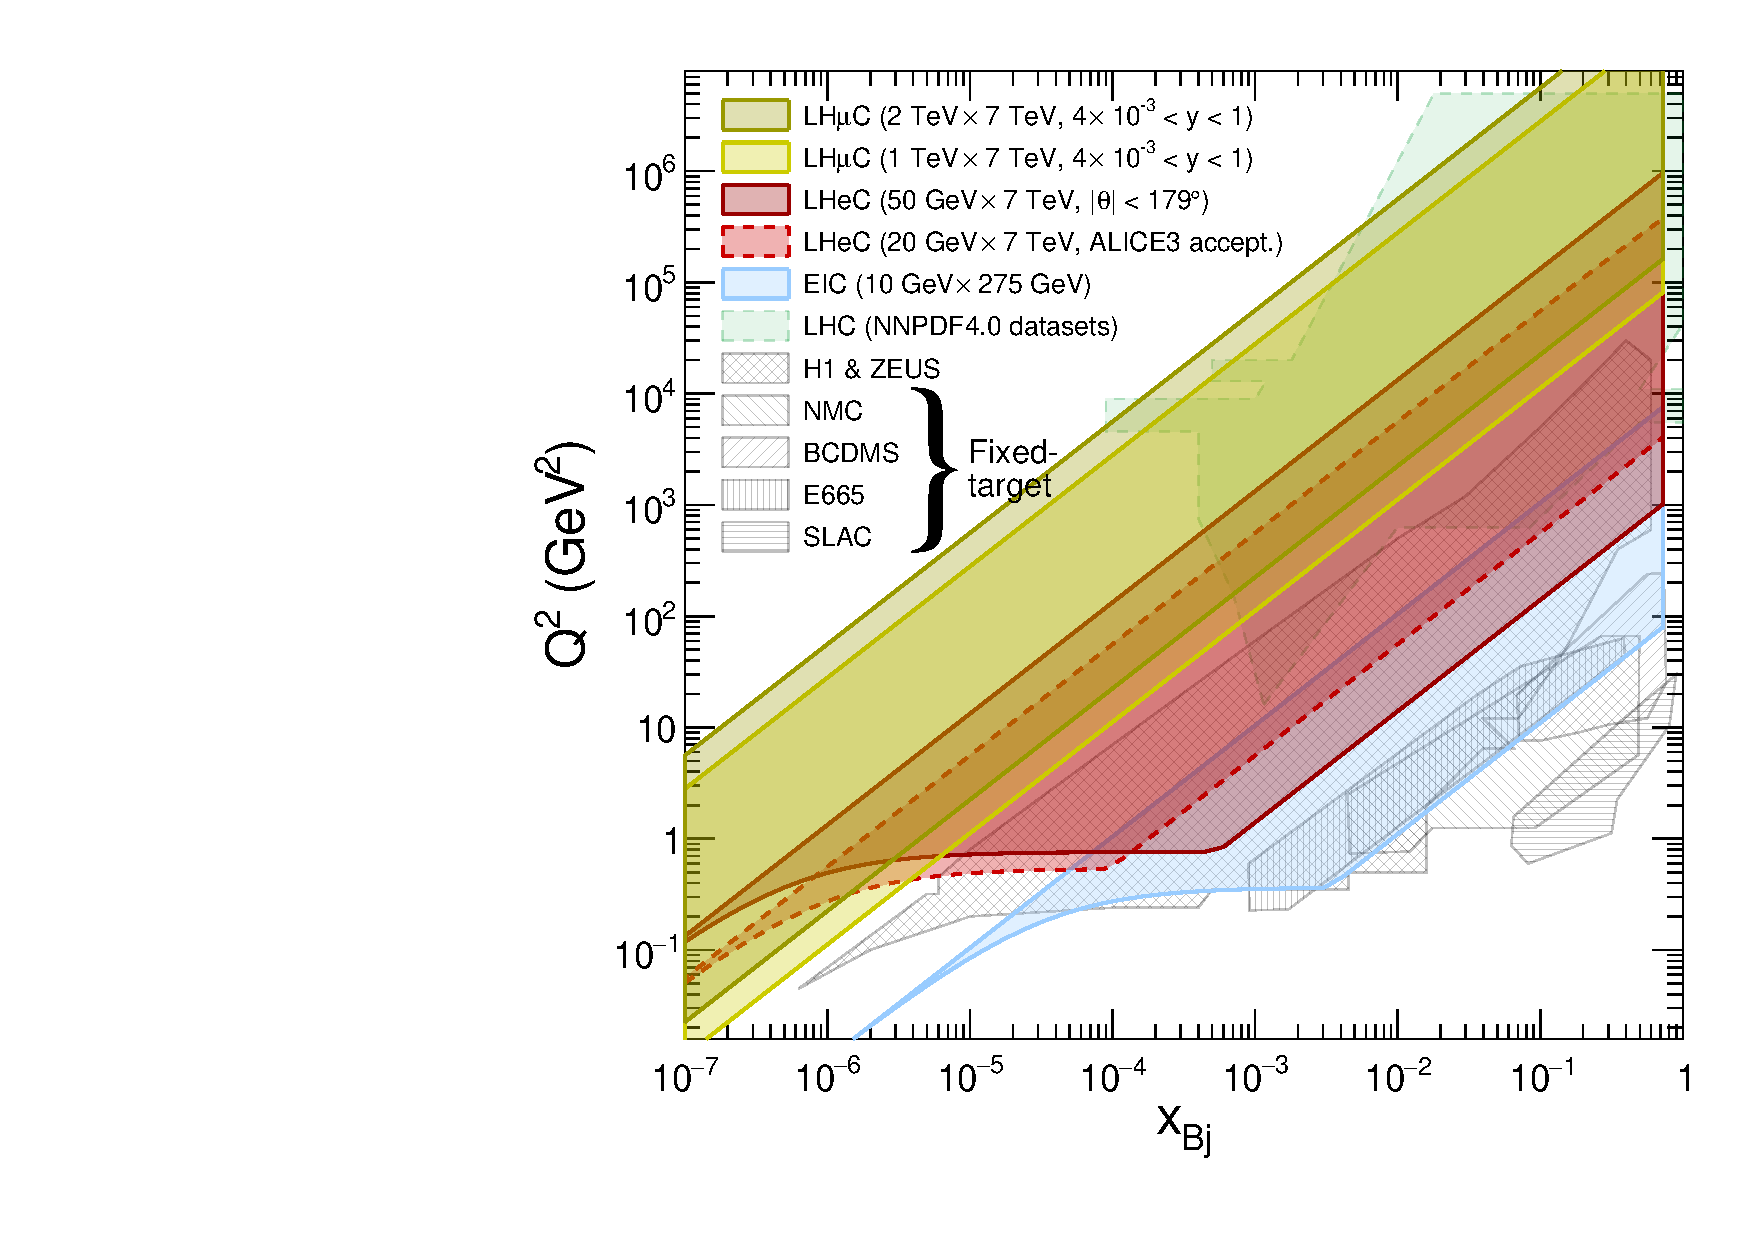
\includegraphics[width=0.55\textwidth]{figures/dis_eta_acceptance.pdf}
\caption{Accessible $(x_{\mathrm{Bj}},Q^2)$ plane from HELP4CERN~\cite{HELP4CERN}, compared with 
existing datasets and planned EIC kinematics. 
The \lhmuc\ regions use $4\times10^{-3}<y<1$. The plotted 20/50~GeV LHeC and 1/2~TeV \lhmuc\ configurations 
retain their original acceptance conventions.}
\label{fig:coverage}
\end{figure}
%-----------------------------------------


%===============================
\section{Higgs production and precision prospects}\label{sec:higgs}
%===============================


The Charged-current (CC) Higgs production proceeds through $W^+W^-$ fusion. 
The channel $\mu^+p\to j\bar\nu_\mu h$ gives an outgoing quark jet, typically forward, 
and missing momentum from the antineutrino. Neutral-current (NC) production, $\mu^+p\to\mu^+jh$, 
proceeds through $ZZ$ fusion and retains the scattered charged lepton. 
Figure~\ref{fig:higgs-production} shows representative partonic contributions. 
These complementary signatures provide access to Higgs interactions with weak bosons; 
extracting couplings also requires decay information and assumptions about the total width. 

\begin{figure}[htbp]
\centering
%---------------- Charged-current production ----------------
\begin{minipage}[t]{0.48\textwidth}
\centering
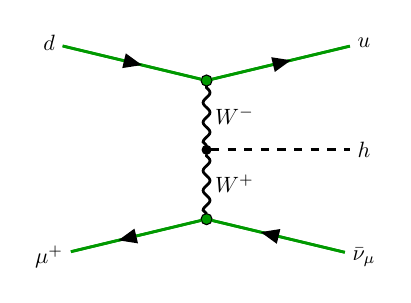
\begin{tikzpicture}[scale=0.80, transform shape]
\begin{feynman}
\vertex (i1) at (-2.5,  1.7) {\(d\)};
\vertex (i2) at (-2.5, -1.7) {\(\mu^{+}\)};
				
\vertex [dot, fill=green!60!black, minimum size=5pt]
(v1) at (0, 1.1) {};
\vertex [dot, fill=green!60!black, minimum size=5pt]
(v2) at (0,-1.1) {};
\vertex [dot, minimum size=4pt]
(m1) at (0,0) {};
				
\vertex (o1) at (2.5,  1.7) {\(u\)};
\vertex (o2) at (2.5, -1.7) {\(\bar{\nu}_{\mu}\)};
\vertex (h1) at (2.5,  0.0) {\(h\)};
				
\diagram*{
(i1) -- [fermion, draw=green!60!black, line width=1pt] (v1)
-- [fermion, draw=green!60!black, line width=1pt] (o1),
(i2) -- [anti fermion, draw=green!60!black, line width=1pt] (v2)
-- [anti fermion, draw=green!60!black, line width=1pt] (o2),
(v1) -- [boson, edge label=\(W^{-}\), line width=1pt] (m1),
(m1) -- [boson, edge label=\(W^{+}\), line width=1pt] (v2),
(m1) -- [scalar, line width=1pt] (h1),
};
\end{feynman}
\end{tikzpicture}
		
\smallskip
{\small (a) Charged-current production}
\end{minipage}
\hfill
%---------------- Neutral-current production ----------------
\begin{minipage}[t]{0.48\textwidth}
\centering
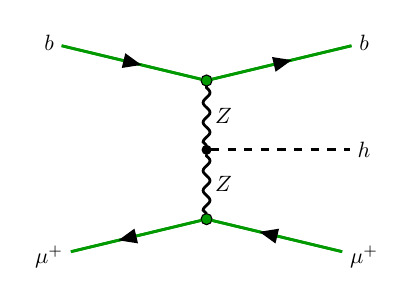
\begin{tikzpicture}[scale=0.80, transform shape]
\begin{feynman}
\vertex (i1) at (-2.5,  1.7) {\(b\)};
\vertex (i2) at (-2.5, -1.7) {\(\mu^{+}\)};
				
\vertex [dot, fill=green!60!black, minimum size=5pt]
(v1) at (0, 1.1) {};
\vertex [dot, fill=green!60!black, minimum size=5pt]
(v2) at (0,-1.1) {};
\vertex [dot, minimum size=4pt]
(m1) at (0,0) {};
				
\vertex (o1) at (2.5,  1.7) {\(b\)};
\vertex (o2) at (2.5, -1.7) {\(\mu^{+}\)};
\vertex (h1) at (2.5,  0.0) {\(h\)};
				
\diagram*{
(i1) -- [fermion, draw=green!60!black, line width=1pt] (v1)
-- [fermion, draw=green!60!black, line width=1pt] (o1),
(i2) -- [anti fermion, draw=green!60!black, line width=1pt] (v2)
-- [anti fermion, draw=green!60!black, line width=1pt] (o2),
(v1) -- [boson, edge label=\(Z\), line width=1pt] (m1),
(m1) -- [boson, edge label=\(Z\), line width=1pt] (v2),
(m1) -- [scalar, line width=1pt] (h1),
};
\end{feynman}
\end{tikzpicture}
		
\smallskip
{\small (b) Neutral-current production}
\end{minipage}

\caption{Representative tree-level diagrams for Higgs production
in positive-muon--proton collisions:
(a) the charged-current subprocess
$\mu^+d\to\bar\nu_\mu uh$ through $W^+W^-$ fusion;
(b) the neutral-current subprocess
$\mu^+b\to\mu^+bh$ through $ZZ$ fusion.
The outgoing
quark contributes to the jet signature. }
\label{fig:higgs-production}
\end{figure}
%----------------------------------





%===============================
\subsection{A dedicated \texorpdfstring{$h\to b\bar b$}{h to bb} study}\label{subsec:htobb}
%===============================


Following the approach of Ref.~\cite{Cheung:2021iev}, we study $\mu^+p\to j\bar\nu_\mu h$, $h\to b\bar b$, 
against CC multijet production and weak-boson-fusion $Z\to b\bar b$. 
We use an LHeC-like Delphes detector simulation~\cite{deFavereau:2013fsa}, a 75\% $b$-tagging factor, 
exactly two selected $b$-jets, and $|m_{bb}-m_h|<25~\mathrm{GeV}$. 
The statistical rate uncertainty is given by, 

%-----------------------------------------
\begin{equation}
\frac{\Delta\sigma}{\sigma}=\frac{\sqrt{N_s+N_b}}{N_s},
\label{eq:stat}
\end{equation}
%-----------------------------------------

where $N_s$ and $N_b$ are selected signal and background counts. 
The calculated precisions are $1.19\%$ and $0.69\%$ for the 500~GeV and 1~TeV studies, respectively~\cite{HELP4CERN,Khanpour:DIS2026}. 

The bottom-Yukawa extraction uses external information on $R=g_{hWW}^2/\Gamma_h$, 
where $\Gamma_h$ is the total Higgs width. 
Since $\sigma(\mu^+p\to j\bar\nu_\mu h)\,\mathrm{BR}(h\to b\bar b)\propto R\,g_{hbb}^2$, 
independent relative uncertainties are combined as

%-----------------------------------------
\begin{equation}
\frac{\Delta g_{hbb}}{g_{hbb}}
=\frac12\sqrt{\left(\frac{\Delta\sigma}{\sigma}\right)^2+
\left(\frac{\Delta R}{R}\right)^2}.
\label{eq:coupling}
\end{equation}
%-----------------------------------------

With $\Delta R/R=0.985\%$ following the FCC-ee benchmark treatment of Ref.~\cite{Cheung:2021iev}, 
the calculated coupling precisions are $0.77\%$ and $0.60\%$. The analysis thus illustrates 
subpercent bottom-Yukawa sensitivity, conditional on the external input and 
statistical treatment, rather than a complete experimental uncertainty forecast.



%===============================
\subsection{Exploratory combined coupling fit}\label{subsec:combined-coupling-fit}
%===============================


Figure~\ref{fig:higgs-couplings} summarizes the complementary 
$\kappa$-3 fit~\cite{HELP4CERN,deBlas:2019rxi}, implemented in SMEFiT~\cite{Armadillo:2026mvp}. 
The study rescales the statistical components of the LHeC 
signal-strength uncertainties using production rates while retaining the 
background, acceptance, efficiency and systematic-factor assumptions. 

%-----------------------------------------
\begin{figure}[tbp]
\centering
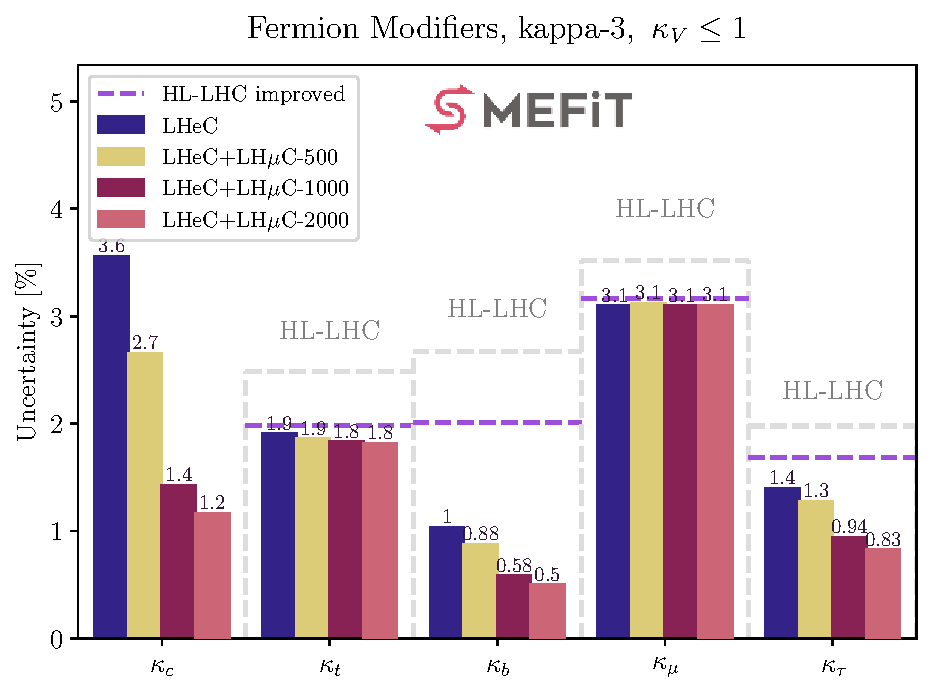
\includegraphics[width=.49\textwidth]{figures/LHmuC_fermion.pdf}\hfill
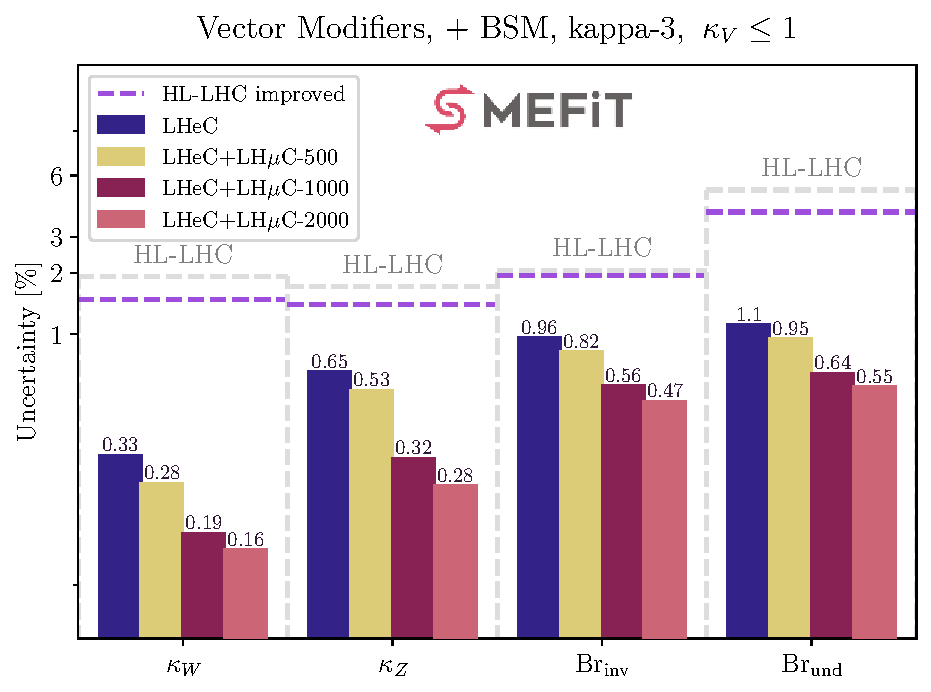
\includegraphics[width=.49\textwidth]{figures/LHmuC_vector.pdf}
\par\smallskip
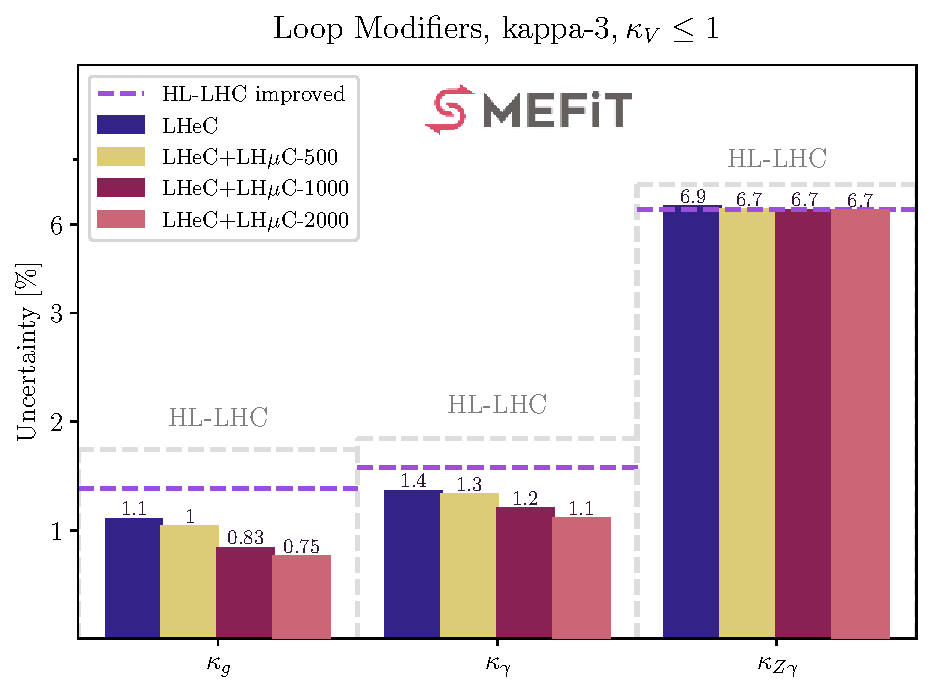
\includegraphics[width=.49\textwidth]{figures/LHmuC_loop.pdf}
\caption{Exploratory $\kappa$-3 fit projections from
HELP4CERN~\cite{HELP4CERN}: fermion modifiers (upper left), vector modifiers and 
invisible/undetected branching fractions (upper right), and effective loop-induced 
modifiers (lower). The legend identifies the LHeC and combined LHeC+\lhmuc\ stages; 
dashed lines show HL-LHC baselines. Coupling uncertainties and absolute branching-fraction 
constraints are in percent. The fit imposes $\kappa_V\le1$, with the vector 
convention defined in the text.}
\label{fig:higgs-couplings}
\end{figure}
%-----------------------------------------

Relative to the plotted LHeC reference, the combination with 
the 1~TeV \lhmuc\ stage reduces the $\kappa_W$, $\kappa_Z$ and $\kappa_b$ uncertainties 
from $0.33\%$, $0.65\%$ and $1.00\%$ to $0.19\%$, $0.32\%$ and $0.58\%$, respectively; 
the $\kappa_c$ uncertainty decreases from $3.6\%$ to $1.4\%$. 
The combined 500~GeV and 2~TeV stages give $\kappa_W$ uncertainties of $0.28\%$ and $0.16\%$, 
respectively, while the 2~TeV results reach $0.50\%$ for $\kappa_b$ and $1.2\%$ for $\kappa_c$. 
At 2~TeV, the $\kappa_g$ and $\kappa_\gamma$ uncertainties reach $0.75\%$ and $1.1\%$. 
The improvement is channel dependent, with smaller changes in $\kappa_t$, $\kappa_\mu$ and $\kappa_{Z\gamma}$. 
The HL-LHC baselines~\cite{ATLAS:2025eii} show the complementary role of these constraints; 
the ``improved'' baseline includes reduced proton PDF and $\alpha_s$ uncertainties~\cite{Ahmadova:2025vzd}. 
Comparisons depend on the width and exotic-decay treatment: the HL-LHC reference study 
assumes the SM Higgs width and no BSM branching fraction, whereas this fit allows 
invisible and undetected modes subject to $\kappa_V(\kappa_W,\kappa_Z)\le1$. 
Its vector uncertainty is defined as $1-\kappa_V(68\%)$. These are exploratory combined 
projections, distinct from standalone \lhmuc\ sensitivities and the dedicated $h\to b\bar b$ extraction.




%===============================
\section{Electroweak and top physics}\label{sec:ewtop}
%===============================

The extended DIS range provides access to electroweak interactions at higher momentum transfer. 
NC and CC measurements probe different flavour and coupling combinations, 
motivating studies of the running weak mixing angle, electroweak parameters 
such as $M_W$, and effective interactions~\cite{HELP4CERN,LHeC:2020van}. 
The top-production gains in Table~\ref{tab:rates} make this programme particularly compelling. 
For the nominal $1~\mathrm{ab}^{-1}$ sample, its cross-sections correspond to 
approximately $3.7\times10^7$ produced single-top events and $2.2\times10^6$ top-pair events, 
before decays, acceptance and selection. CC single-top production probes the charged-current 
top interaction and motivates $Wtb$ and CKM studies, while NC top-pair production supplies 
complementary production and decay observables~\cite{HELP4CERN}. The distinct lepton-hadron environment 
complements the large HL-LHC samples through different initial states and 
systematic sensitivities, rather than a universal advantage in event counts. 
Rare decays such as $t\to q\gamma$, $qZ$ and $qH$, with $q=u,c$, provide further 
directions for dedicated analyses. Quantitative limits require reconstructed observables, 
backgrounds and correlated uncertainties. 
Although low pileup is advantageous, a realistic assessment of
detector-level performance requires detailed detector simulations
and comprehensive background studies~\cite{HELP4CERN}. 


%===============================
\section{Photon-induced physics}\label{sec:photon}
%===============================


Quasi-real photons radiated by the lepton and proton provide an additional production mechanism~\cite{Budnev:1974de,Forthomme:DIS2024,HELP4CERN}. 
In the equivalent-photon approximation (EPA)~\cite{Budnev:1974de},
the effective photon-photon luminosity $S_{\gamma\gamma}(W)$ is folded
with the subprocess cross section to obtain the total inclusive
cross section at the lepton-proton level: 

%-----------------------------------------
\begin{equation}
\sigma(\mu^+p\to\mu^+Xp;W>W_0)
=\int_{W_0}^{W_{\mathrm{max}}}dW\,S_{\gamma\gamma}(W)\,
\hat\sigma(\gamma\gamma\to X;W).
\label{eq:epa}
\end{equation}
%-----------------------------------------

Here $W$ is the photon-pair invariant mass, distinct from $\sqrt{s_{\mu p}}$, 
and $W_{\mathrm{max}}$ is its kinematic endpoint. 
Figure~\ref{fig:photon} shows the elastic photon-photon luminosity 
and inclusive $\tau$-pair production rates at the LHeC and LH$\mu$C.
For $W_0=10~\mathrm{GeV}$, the reported $\tau^+\tau^-$ 
cross-sections are $50.37$, $58.56$ and $70.3$~pb for 50~GeV electrons, 
500~GeV muons and 1~TeV muons, respectively, on 7~TeV protons~\cite{HELP4CERN,Khanpour:DIS2026}. 
For the same configurations, elastic $W^+W^-$ production above threshold gives $0.037$, $0.166$ and $0.258$~pb. 
The latter represents enhancements of approximately 4.5 and 7 over the LHeC benchmark, 
illustrating the stronger benefit for heavier final states. 

%-----------------------------------------
\begin{figure}[htbp]
\centering
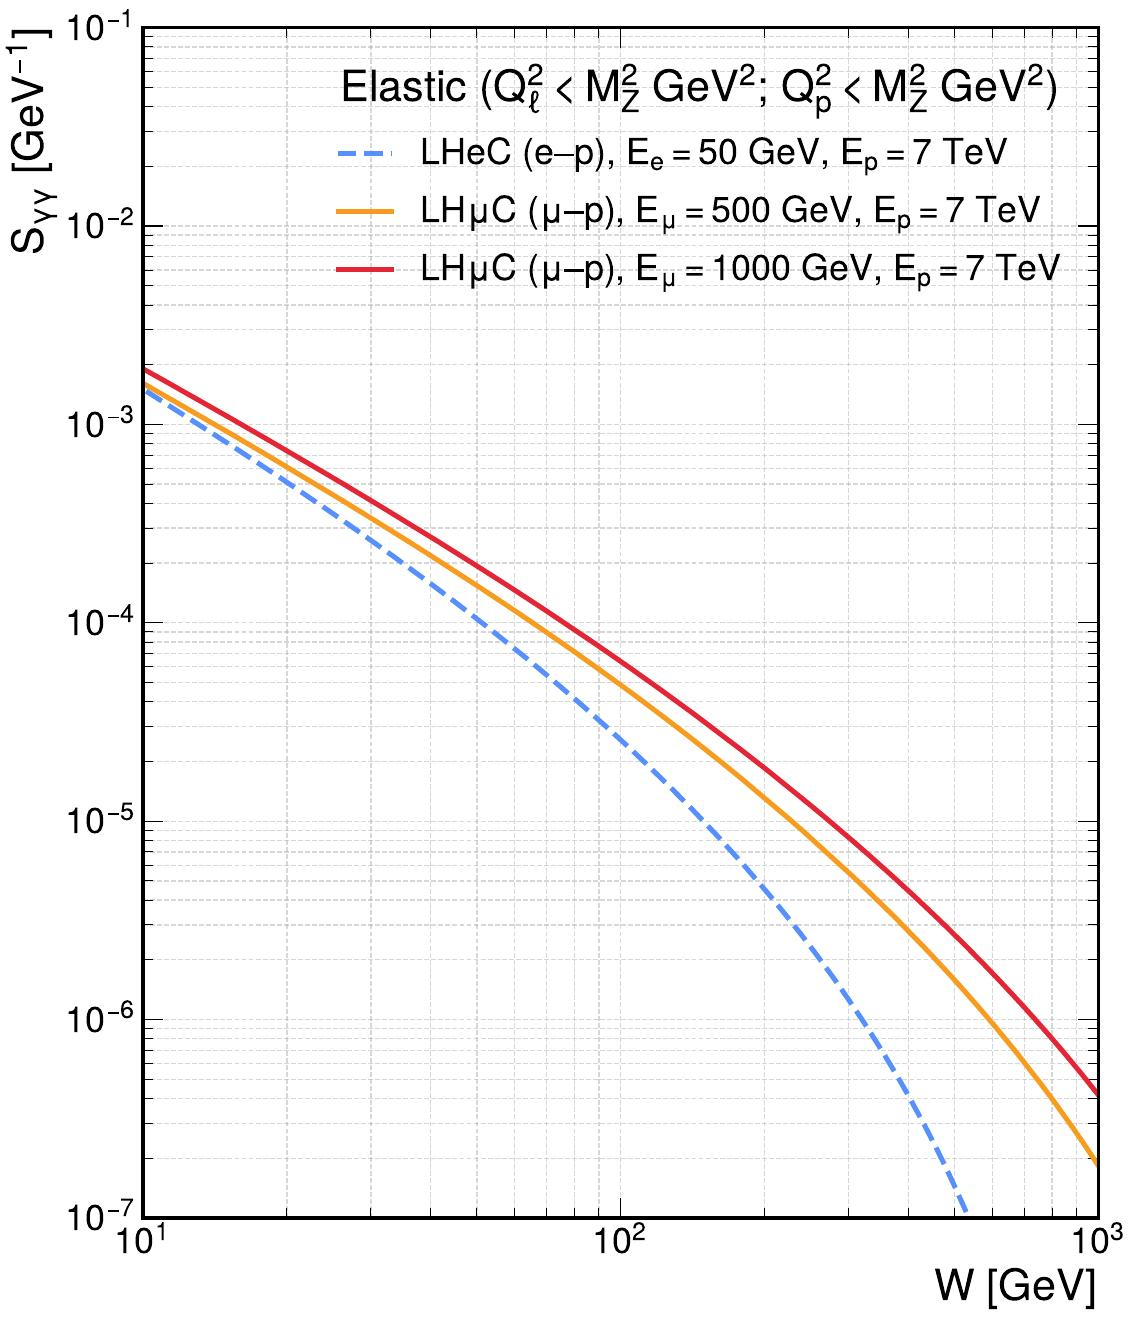
\includegraphics[width=0.40\textwidth]{figures/Sgg.jpg}\hfill
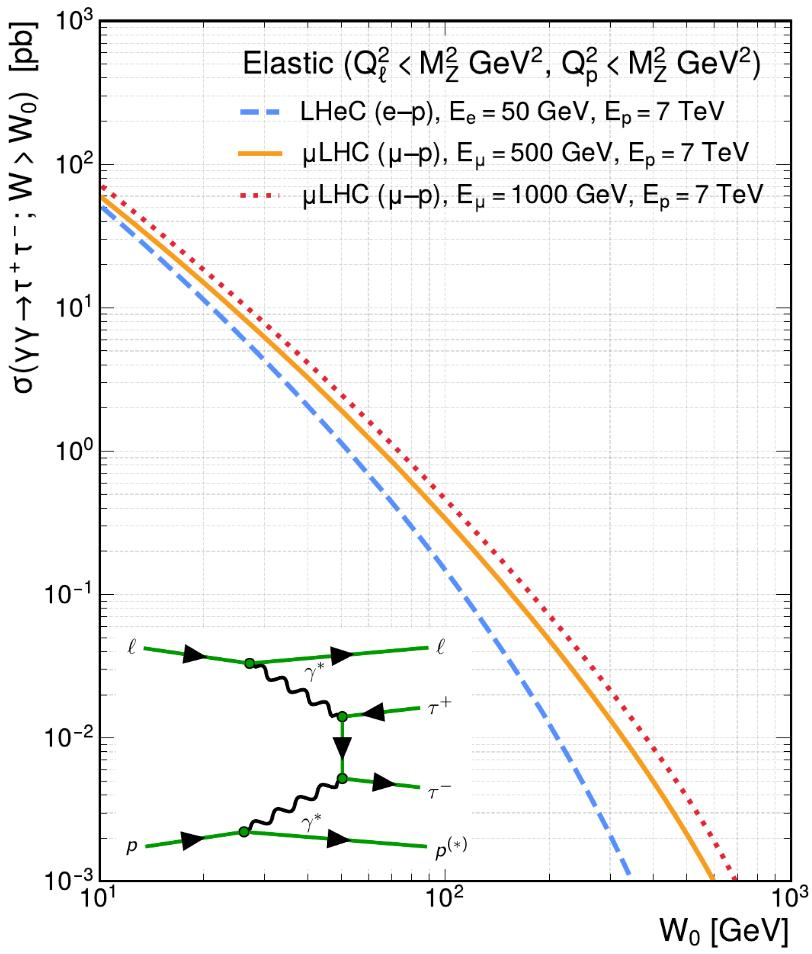
\includegraphics[width=0.40\textwidth]{figures/yytautau.jpg}
\caption{The elastic photon luminosity (left) and cumulative $\tau$-pair 
cross-section $\sigma(W>W_0)$ (right) at the LHeC and LH$\mu$C~\cite{Khanpour:DIS2026}.}
\label{fig:photon}
\end{figure}
%-----------------------------------------


The $\gamma\gamma$ programme also includes loop-induced $\gamma\gamma\to ZZ$, top-pair production, 
and charged BSM pairs such as higgsino-like states and sleptons~\cite{HELP4CERN,Khanpour:DIS2026}. 
The heavier SM channels have smaller, fb-scale rates and require dedicated sensitivity studies. 
High-mass distributions offer probes of tau electromagnetic properties 
and gauge-boson interactions. 





%===============================
\section{BSM perspectives}\label{sec:BSM}
%===============================


Muon-parton interactions provide a further source of complementarity with proton colliders. 
We consider resonant squark production through $R$-parity-violating $\mu q$ interactions 
and color-octet muon (leptogluon) production through a $\mu g$ interaction~\cite{HELP4CERN,Cheung:2021iev}. 
In the studied RPV scenarios, the NC channel benefits from a valence-quark initial state relative 
to the sea-quark CC channel. For color-octet muons, resonant single production 
at \lhmuc\ complements QCD pair production at the HL-LHC. 
These mechanisms probe the muon coupling directly; their mass reach depends on 
couplings, the compositeness scale where applicable, luminosity and event selection, 
rather than on collision energy alone. 



%===============================
\section{Conclusions}\label{sec:outlook}
%===============================

The \lhmuc\ working points extend the CERN lepton-hadron programme to 3.7--7.5~TeV and 
provide substantial gains in heavy-particle production over the adopted LHeC benchmarks. 
The dedicated $h\to b\bar b$ study illustrates subpercent bottom-Yukawa sensitivity with 
external coupling/width information, while the exploratory combined fit improves the   
LHeC vector and fermion constraints, reaching $0.19\%$ for $\kappa_W$ at the nominal 
stage under $\kappa_V\le1$. Enhanced top production, heavier photon-induced final states 
and resonant muon-parton channels broaden the physics case. 
Together with the complementary HL-LHC measurements, these results motivate a 
coordinated programme of Higgs, electroweak, top and new-physics studies, supported by 
dedicated detector and systematic analyses. 

\begin{thebibliography}{99}

\bibitem{Akturk:2025ubm}
D.~Akturk et al., \emph{$\mu$LHC: Antimuon Ring and High Luminosity-LHC-Based $\mu^+p$ Collider},
\href{https://doi.org/10.1093/ptep/ptag031}{PTEP \textbf{2026}, 033C04},
\href{https://arxiv.org/abs/2506.15445}{arXiv:2506.15445}.



\bibitem{LHeC:2020van}
P.~Agostini et al. [LHeC and FCC-he Study Group], \emph{The Large Hadron--Electron Collider at the HL-LHC},
\href{https://doi.org/10.1088/1361-6471/abf3ba}{J. Phys. G \textbf{48} (2021) 110501},
\href{https://arxiv.org/abs/2007.14491}{arXiv:2007.14491}.



\bibitem{Ahmadova:2025vzd}
F.~Ahmadova et al., \emph{The Large Hadron electron Collider as a bridge project for CERN},
\href{https://arxiv.org/abs/2503.17727}{arXiv:2503.17727}.



\bibitem{Khanpour:DIS2026}
H.~Khanpour, \emph{Perspectives for HET physics studies at a muon-hadron collider at CERN},
\href{https://agenda.infn.it/event/47074/contributions/289107/}{presentation at DIS2026},
Bologna, 7 May 2026.



\bibitem{HELP4CERN}
HELP4CERN Study Group, \emph{White Paper on High Energy, High Luminosity Lepton-Hadron Colliders at CERN},
supplied working draft, in preparation.



\bibitem{Andre:2025iar}
K.~D.~J.~Andr{\'e}, L.~Forthomme, B.~Holzer and K.~Piotrzkowski,
\emph{An electron--hadron collider at the high-luminosity LHC},
\href{https://doi.org/10.1088/1367-2630/ae2e31}
{New J. Phys. \textbf{28}, no.~1, 013001 (2026)},
\href{https://arxiv.org/abs/2503.20475}
{arXiv:2503.20475 [hep-ex]}.


\bibitem{Cheung:2021iev}
K.~Cheung and Z.~S.~Wang, \emph{Physics potential of a muon-proton collider},
\href{https://doi.org/10.1103/PhysRevD.103.116009}{Phys. Rev. D \textbf{103} (2021) 116009},
\href{https://arxiv.org/abs/2101.10476}{arXiv:2101.10476}.



\bibitem{deFavereau:2013fsa}
J.~de Favereau et al. [DELPHES 3], \emph{DELPHES 3, A modular framework for fast simulation of a generic collider experiment},
\href{https://doi.org/10.1007/JHEP02(2014)057}{JHEP \textbf{02} (2014) 057},
\href{https://arxiv.org/abs/1307.6346}{arXiv:1307.6346}.




\bibitem{deBlas:2019rxi}
J.~de Blas et al., \emph{Higgs Boson Studies at Future Particle Colliders},
\href{https://doi.org/10.1007/JHEP01(2020)139}{JHEP \textbf{01} (2020) 139},
\href{https://arxiv.org/abs/1905.03764}{arXiv:1905.03764}.




\bibitem{Armadillo:2026mvp}
T.~Armadillo et al., \emph{New Physics Reach through Precision at Future Colliders: a Multi-Pronged Approach},
\href{https://arxiv.org/abs/2604.16596}{arXiv:2604.16596}.



\bibitem{ATLAS:2025eii}
ATLAS and CMS Collaborations, \emph{Highlights of the HL-LHC physics projections by ATLAS and CMS},
\href{https://arxiv.org/abs/2504.00672}{arXiv:2504.00672}.



\bibitem{Budnev:1974de}
V.~M.~Budnev, I.~F.~Ginzburg, G.~V.~Meledin and V.~G.~Serbo,
\emph{The two-photon particle production mechanism. Physical problems. Applications. Equivalent photon approximation},
\href{https://doi.org/10.1016/0370-1573(75)90009-5}{Phys. Rept. \textbf{15} (1975) 181}.



\bibitem{Forthomme:DIS2024}
L.~Forthomme, H.~Khanpour, K.~Piotrzkowski and Y.~Yamazaki,
\emph{High energy $\gamma\gamma$ interactions at the LHeC},
\href{https://doi.org/10.22323/1.469.0269}{PoS(DIS2024)269 (2025)}.


\end{thebibliography}



\end{document}


